\chapter{DISCUSSION}

In this work, genome-scale metabolic modelling methods are used to analyze transcriptomics of evolved \emph{S. cerevisiae} strains that have been obtained by in vivo evolutionary engineering strategies for different environmental conditions where the following substances are gradually increased in the media: Ethanol\cite{turanli2017vivo}, caffeine\cite{surmeli2019evolutionary}, coniferyl aldehyde\cite{hacisalihouglu2019genomic}, iron\cite{balaban2020evolutionary}, nickel\cite{kuccukgoze2013evolutionary}, phenylethanol\cite{holyavkin2013evrimsel}, and silver\cite{terziouglu2020genomic}. Overall workflow of the study is described Figure \ref{fig:methods}.


\begin{figure}[H]
  \begin{center}
  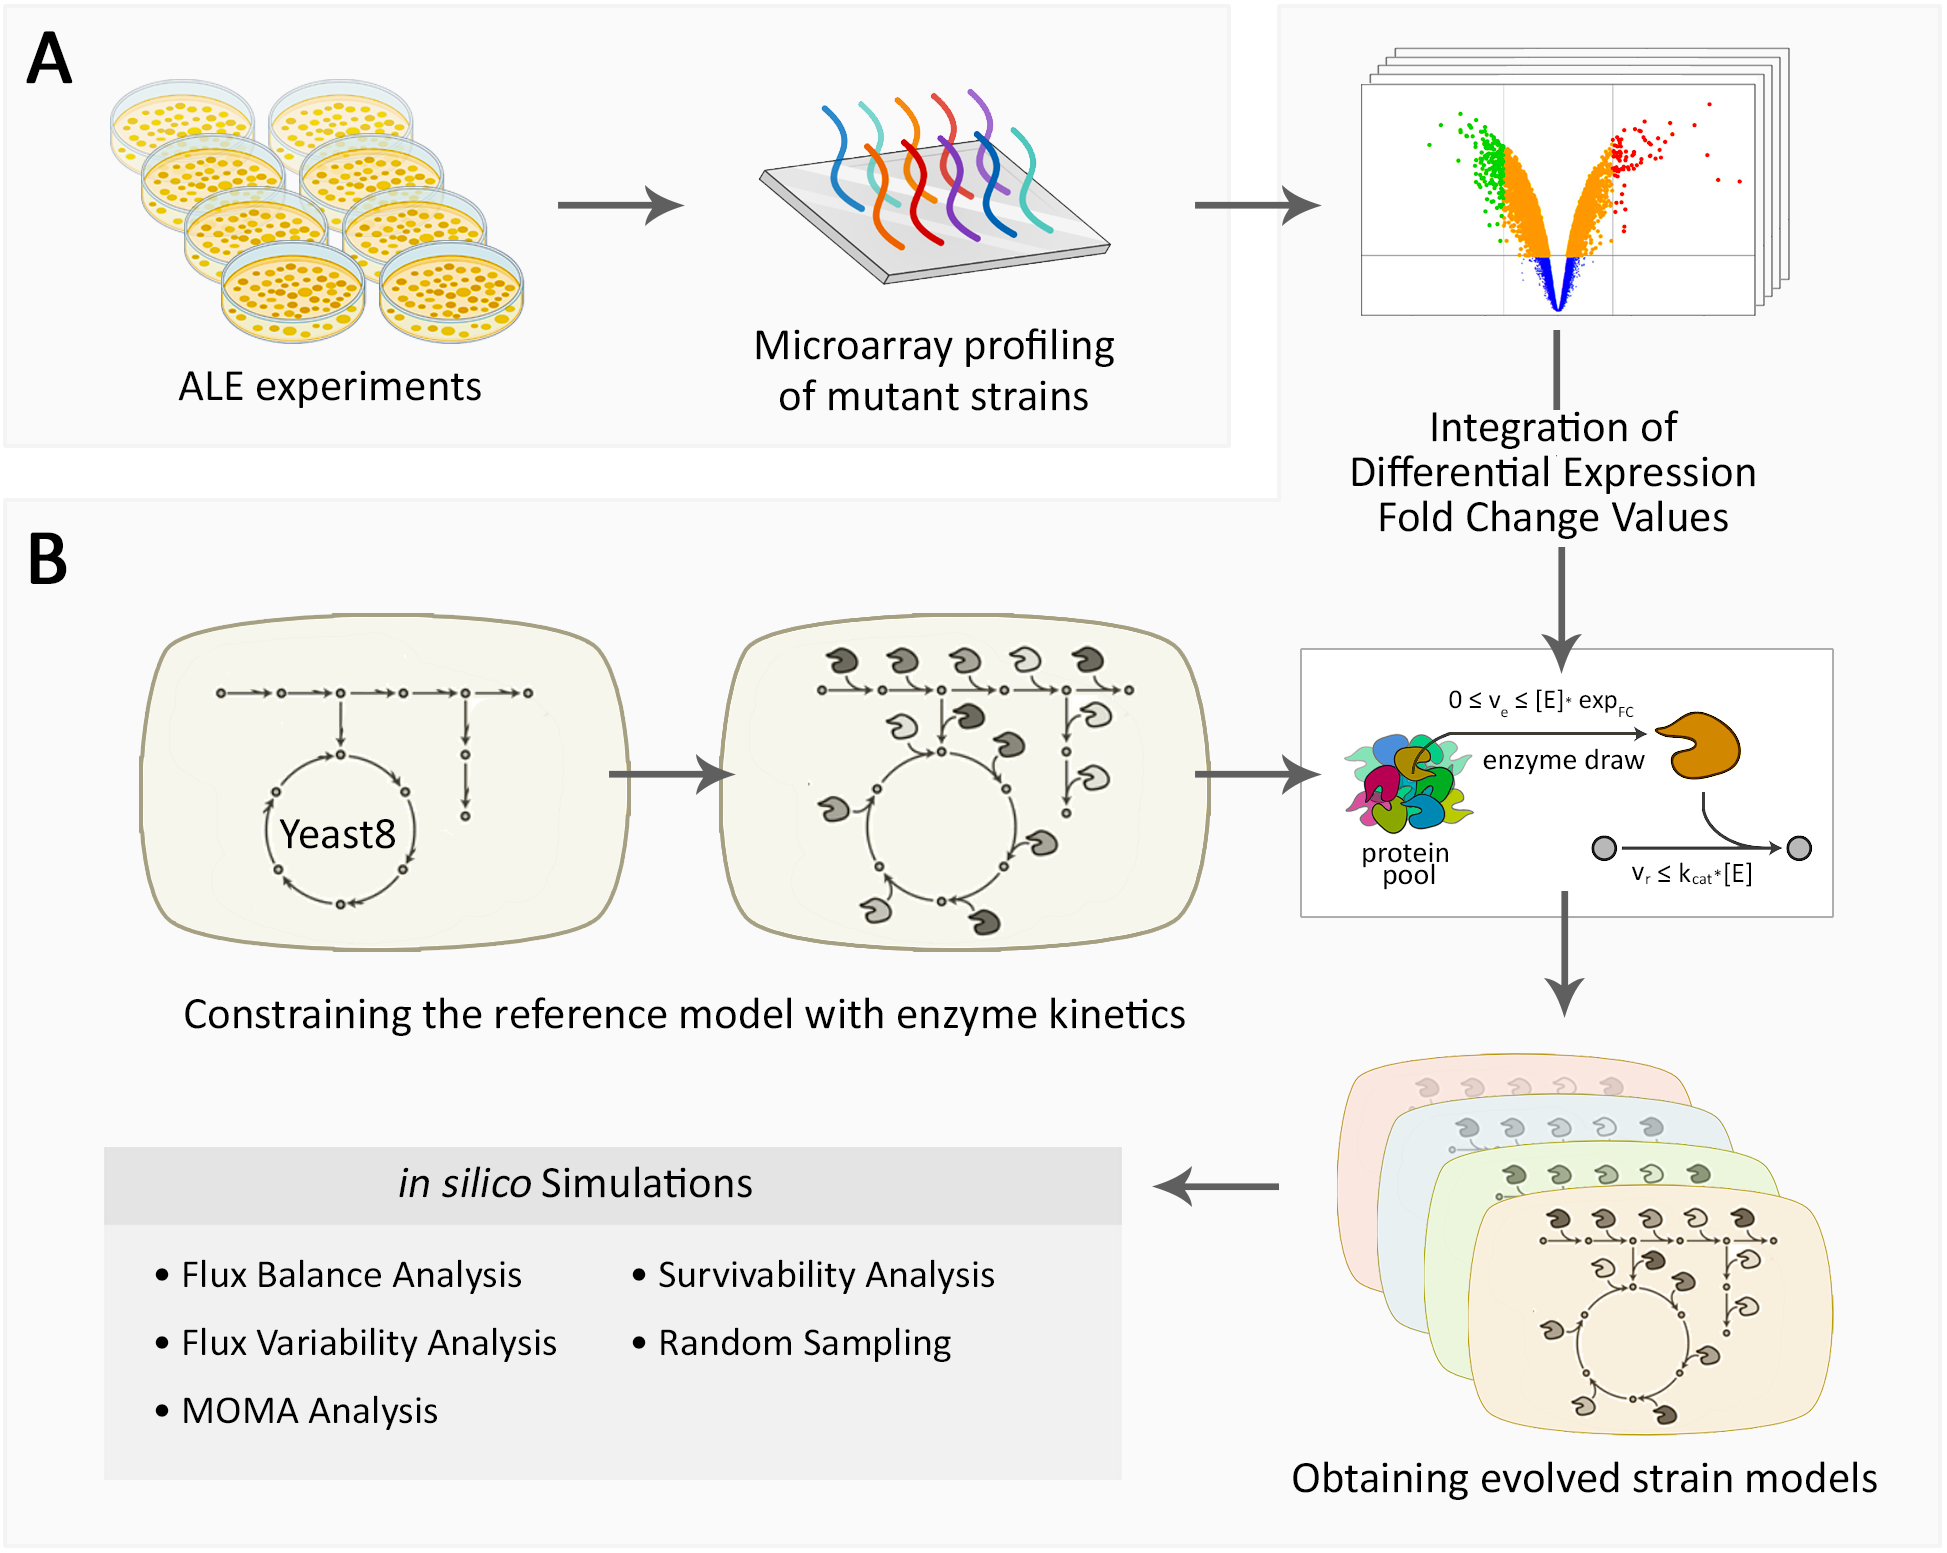
\includegraphics[width=1\columnwidth]{figures/methods_vert.png}
  \caption[Overall workflow of the study: A) preprocessed microarray and experimental data on evolved strains are obtained from Cakar's Lab, B) model reconstruction and \emph{in silico} analyses are carried out.]{Overall workflow of the study: A) preprocessed microarray and experimental data on evolved strains are obtained from Cakar's Lab, B) model reconstruction and \emph{in silico} analyses are carried out. }
  \label{fig:methods}
  \end{center}
\end{figure}

\section{Flux Distribution Comparisons}
FBA and robustness analyses where growth rates are maximized against varying levels of glucose uptake and oxygen uptake rates predicted non-linear robustness graphs. This non-linearity shows that the reconstructed metabolic models which are used in this study were able to simulate overflow metabolism without the \emph{ad hoc} constraints.

By simulating the varying the carbon concentration in the media, a transition region that is known as Janusian region is predicted \cite{buttonbiochemical}. Using enzymatic constraints with GECKO methodology helps us to capture this region since it occurs when the cells are limited in nutrient and protein availability-wise. In the analyses, this region is observed for growth rates above 0.3 h\textsuperscript{-1} in all strains as the metabolic enzymes became saturated due to protein pool limitation.

Evolved strains produce biomass at different rates, with different exchange metabolite preferences due to their non-identical protein availability. Caffeine resistant strain reaches the highest growth rate amongst evolved strains, and the strain was able to maintain its energy without using the oxidative phosphorylation pathway and it is highly sensitive to oxygen levels in the media. Simulations show that the strain cannot grow at all if the oxygen uptake rate is higher than 25 mmol (gDW)\textsuperscript{-1} h\textsuperscript{-1} and if enough carbon is available in the media to uptake, cells prefer to simulate hypoxia in order to produce biomass at higher rates. However, when the carbon source is limited, cells prefer to take more oxygen inside the cell. On the other hand, silver resistant strain which is the most distinguished evolved strain next to caffeine resistant strain, had the lowest maximum $\mu$ but it was able to produce biomass at higher rates under higher oxygen and glucose uptake rates compared to other strains.

Multiple \emph{in silico} analyses showed that, although the predictions for the glucose uptake and ATP production rates of silver resistant strain is high, the strain does not carry fluxes through oxidative phosphorylation, in mitochondria. When total flux values through the reactions of coenzymes NAD, NADP, FAD and glutathione system are investigated, an outstanding difference on the glutathione metabolism activity is observed. It has previously shown in the literature that glutathione metabolism is highly connected with stress response mechanisms, and glutathione itself has a role in the maintenance of cellular structure integrity \cite{penninckx2002overview}. With that information, the change in the glutathione metabolism of silver resistant strain could be further investigated in stress response coupled with adaptive evolution. SEC53, a phosphomannomutase which localizes to cytoplasmic stress granules also a stress related response\cite{kepes1988yeast} and its activity is decreased notably in phenylethanol resistant strain.

Another noteworthy metabolite, riboflavin, has a monofunctional role in FMN and FAD biosynthesis pathways \cite{oltmanns1972biosynthesis}. Phenylethanol resistant strain showed decreased activity through riboflavin biosynthesis pathway by RIB7 (2,5-diamino- 6-(ribosylamino)- 4(3H)-pyrimidinone 5'-phosphate reductase) despite its increased activities through TDH1 (glyceraldehyde-3-phosphate dehydrogenase) and OLI1 (F0 ATP synthase subunit c) in MOMA results, directs us to focus on energy utilization pathways.

OLI1, the main transmembrane subunit of F-type ATP synthases, and TIM11, subunit e of mitochondrial F1F0-ATPase take part in the mitochondrial enzyme F0F1-ATPase / ATP synthase synthesizes during oxidative phosphorylation \cite{arnold1997yeast, trembath1975biogenesis}. Changes in the OLI1 and TIM11 activities in the mutant strains  are important to investigate since the ATPase is an evolutionarily conserved enzyme complex \cite{tokatlidis1996translocation}. COB (cytochrome b), a subunit of the mitochondrial respiratory chain complex III (transmembrane cytochrome bc1), catalyzes the quinol oxidation and cytochrome c reduction reactions, meanwhile generating a force to proton motive in ATP synthesis \cite{meunier2013respiratory}. Caffeine, ethanol B8, and phenylethanol resistant strains have increased their activities compared to reference strains, and the silver resistant strain was the only strain which has decreased its flux for COB activity. As protein allocation decides which reactions to catalyze or which pathways to activate in cells, these differential findings are useful for analysis of energy metabolism in evolved strains.

A common change between all evolved strains of decreasing glycerol-3-phosphate or dihydroxyacetone phosphate sn-1 acyltransferase (GPT2) activity is observed, except the nickel resistant strain. However, since only a few expression data integrated in the reconstruction of nickel resistant strain, its exception could be ignored in terms of finding a commonality between all strains. GPT2 has a role in the phospholipid biosynthesis, where it catalyzes the acylation of glycerol-3-phosphate and dihydroxyacetone \cite{athenstaedt1997biosynthesis}, and it is one of the main targets.

Two of five related enzymes of the 5-phospho-ribosyl-1(alpha)-pyrophosphate synthetases (PRSs), namely PRS1 and PRS2, were found as another important targets by MOMA as their flux values for each evolved strain differed. Although the flux values of the two enzymes' usages were equal for the reference strain; ethanol B8, caffeine, iron and phenylethanol resistant strains did not carry any fluxes through the enzyme PRS2 and only used the enzyme PRS1 for their activity (caffeine and phenylethanol resistant strains carried low fluxes through PRS1). On the contrary, only the silver resistant strain preferred to use PRS2, and carried zero flux through PRS1.

Phosphoribosyl pyrophosphate (PRPP), synthesized from PRPs, is a key compound in central carbon and nitrogen metabolism, as it has a role in purine, pyrimidine, and pyridine nucleotides synthesis pathways \cite{jimenez2008phosphoribosyl}. A previous study by Schneiter et. al. investigated the five genes of PRSs (PRS1–PRS5), and reported that the $\Delta$prs1 and $\Delta$prs3 mutants of \emph{S. cerevisiae} are hypersensitive to caffeine and they could not survive when exposed to caffeine \cite{schneiter2000importance}. It was also found that PRPP plays a key role in cell wall integrity pathway and cell viability through stress signaling \cite{ugbogu2013contribution}. Here, the caffeine resistant strain carried zero flux through PRS2, and 7.10 fold decreased flux compared to the reference strain. Differential expression analysis also concluded that the caffeine stress causes downregulation on all PRS genes.

Acyltransferase of the glycerolipid biosynthesis pathway, namely SCT1, was inactive in the reference strain's FBA results. However, although the MOMA methodologically finds the solution vector for the evolved strain where the distance between the evolved strain to the reference strain's solution is minimum, SCT1 was activated in ethanol B2, ethanol B8, caffeine, coniferyl aldehyde, and iron resistant strains. It was previous shown in the literature that SCT1 deletion decreases the saturated fatty acid content in the cells, and its overexpression (which was the case for the ethanol B8, coniferyl aldehyde and phenylethanol resistant strains) cause a decrease in desaturation of fatty acids dramatically, and therefore affecting the phospholipid composition of the cells \cite{de2012yeast}.

The followings are found as the most sensitive metabolites from the shadow prices (the derivatives of the objective function, i.e. growth, with respect to the exchange flux of the metabolite, see Table \ref{table:fba_shadowprices_free_table}) in FBA: lanosterol, hexanoate, 14-demethyllanosterol, zymosterol, ergosta-5,7,24(28)-trien-3beta-ol, ergosterol, 4-aminobenzoate, 5-formyltetra hydrofolic acid, flavin mononucleotide (FMN), riboflavin, and biotin.

It is known that the acetyl-coenzyme A carboxylase is a biotin-dependent enzyme, and biotin is also involved in the generation of malonyl-CoA in fatty acid synthesis amongst its many other functionalities \cite{hasslacher1993acetyl, morris1987yeast}. Sensitivity of silver resistant strain to biotin availability has increased almost 2.5 fold whereas caffeine, nickel and phenylethanol resistant strains decreased their sensitivities down to 4 folds. Flavin mononucleotide (FMN) and its precursor riboflavin (vitamin B2) are the metabolites which evolved strains are most sensitive to their changes, and the values for both metabolites are almost the same because their reactions are formed as chain reactions in the metabolic network. FMN, produced from riboflavin, functions as a prosthetic group for several oxidoreductases, mainly NADH dehydrogenase \cite{tsibris1966studies}. The reactions for ergosterol, a sterol found in the cell membrane, and ergosta-5,7,22,24(28)-tetraen-3beta-ol, the product of ergosterol oxidation, are also chained reactions and therefore have same sensitivity values. Zymosterol, an intermediate in cholesterol biosynthesis, 4-aminobenzoate, an intermediate in folate biosynthesis, and 5-formyltetrahydrofolic acid, a folate coenzyme, are also found as important metabolites in sensitivity analysis.

The most divergent enzyme through all evolved model simulations, glyceraldehyde-3-phosphate dehydrogenase (GAPDH) is an enzyme involved in glycolysis and gluconeogenesis pathways and it is encoded by three genes TDH1, TDH2 and TDH3 (triose-phosphate dehydrogenase; TDH) \cite{boucherie1995differential}. It catalyzes the conversion of glyceraldehyde-3-phosphate to 1,3-bisphospho-D-glycerate during glycolysis and the reverse reaction during gluconeogenesis,
\begin{align}
\begin{split}
\ \text{glyceraldehyde-3-phosphate} + NAD + P \leftrightarrow \\
\ \text{1,3-bisphospho-D-glycerate} + H^+ + NADH
\end{split}
\end{align}
where glyceraldehyde-3-phosphate is converted to 1,3-bisphospho-D-glycerate with the NAD and hydrogen.


In this study, it is found that carried flux through GAPDH is increased by 39\% in caffeine, 13\% in silver, and 11\% in coniferyl aldehyde resistant strain. On the contrary, the carried flux is decreased by 31\% in ethanolb2, 15\% in ethanol B8, and 26\% in iron resistant strain. It is also observed that each evolved model uses different isozyme for the catalytic activity. GAPDH differences are summarized in Figure \ref{fig:discuss_GAPDH}.

For a long time, GAPDH was considered as a housekeeping gene for its constitutively expression in the cell, and commonly used in comparisons of expression data. In 2005, Barber et al. have reported different regulation mechanisms for GAPDH under specific conditions\cite{barber2005gapdh}, and it is later found that the gene is upregulated under hypoxic stress \cite{yang2008effects}. Additional functions in other cellular processes have also been described such as being a chaperone protein in cellular iron homeostasis \cite{sweeny2018glyceraldehyde}. Interestingly, catalytically active TDH enzymes are found in both the cytoplasm and the cell wall.

GAPDH activity is controlled with oxygen availability, and evidence suggests that it may be the sensor of the cell in terms of oxidative stress \cite{chuang2005glyceraldehyde}. In the simulations presented here, oxidative phosphorylation through ATP synthase was totally inactive (zero flux) for the caffeine resistant strain under unconstrained conditions, i.e., unlimited availability for uptake metabolites such as oxygen and glucose. Despite the inactivity, caffeine resistant strain was the highest ATP producer among evolved strains, and the ATP production was through pyruvate kinase and phosphoglycerate kinase activity (Table \ref{table:fba_atp_production}). Similar to caffeine resistant strain, silver resistant strain, too, showed increased activity on GAPDH and carried zero flux through ATP synthase in oxidative phosphorylation. In agreement with the results, ethanholb2, ethanol B8, and iron resistant strains showed decreased activity for GAPDH, and they were the only models that show ATP synthase activity.

\begin{figure}[H]
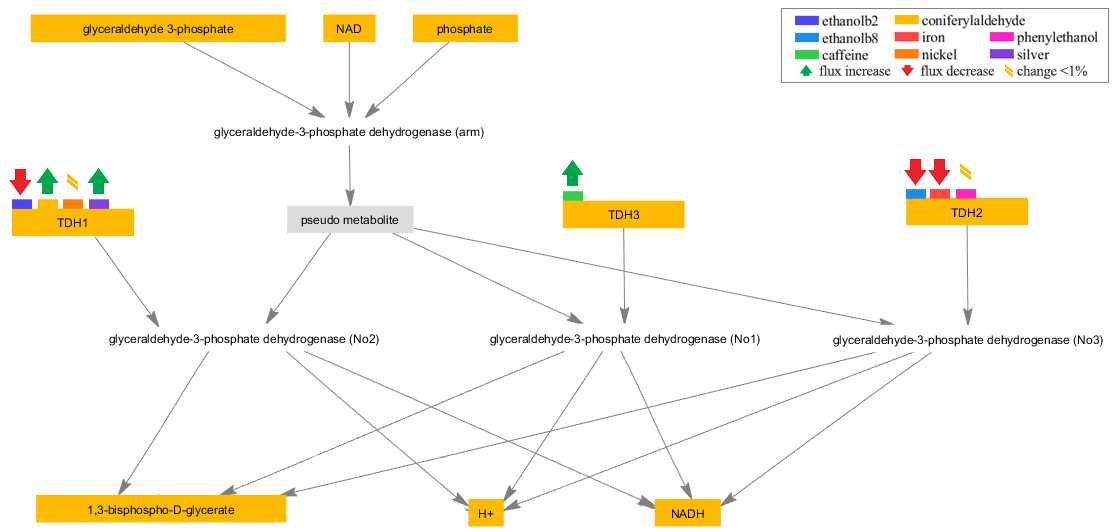
\includegraphics[width=1\columnwidth]{figures/discuss_GAPDH.png}
\caption[Map of glyceraldehyde-3-phosphate dehydrogenase catalyzed reaction as it used in simulations]{Map of glyceraldehyde-3-phosphate dehydrogenase catalyzed reaction as it used in simulations. Corresponding genes used for evolved strains are shown in colors, and flux changes compared to reference strain model simulations are indicated as increased or decreased with arrows.}
\label{fig:discuss_GAPDH}
\end{figure}

\vspace{-1cm}

The most second divergent enzyme through all evolved model simulations is found as pyruvate decarboxylase (PDC), a regulatory component of pyruvate dehydrogenase (PDH) complex that is responsible for conversion of pyruvate to acetyl coenzyme A, therefore making the complex a key metabolic point since it links glycolysis pathway to the TCA cycle. Pyruvate decarboxylase converts pyruvate into acetaldehyde with addition of one proton and release of one molecule of CO$_2$,
\begin{align}
\label{eq:pyrdec}
\ H^+ + pyruvate \rightarrow \text{Acetaldehyde} + \text{carbondioxide}
\end{align}
and this reaction takes places in cytoplasm. Total of three isozymes are used for the pyruvate decarboxylase reaction in the metabolic models: The major of three pyruvate decarboxylases is PDC1 (isozyme 1, encoded by YLR044C), the second most abundant isozyme is PDC5 (isozyme 2, encoded by YLR134W), and lastly, the minor of three pyruvate decarboxylase is PDC6 (isozyme 3, encoded by YGR087C).

In simulations, models chose different isozymes to catalyze pyruvate decarboxylase reaction. While three of them (caffeine,  iron,  phenylethanol models) chose to use PDC5 isozyme, the remaining (ethanolb2, ethanol B8, coniferyl aldehyde, nickel, and silver models) chose PDC1; and none of the models carry fluxes through PDC6 as it can be seen from the Figure \ref{fig:discuss_PDC}. It can be concluded that isozyme preference of models is in agreement with the abundances of isozymes. Additionally, it has been previously reported that the isozyme PDC6 is not used by yeast while the fermentation of glucose is active \cite{hohmann1991pdc6}.

\begin{figure}[H]
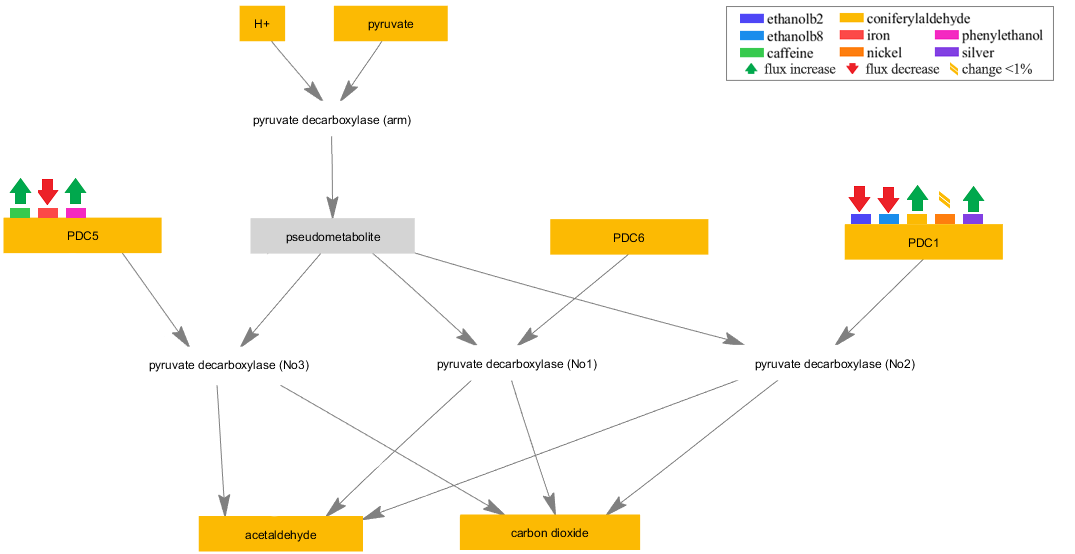
\includegraphics[width=1\columnwidth]{figures/discuss_PDC.png}
\caption[Map of pyruvate decarboxylase catalyzed reaction as it used in simulations]{Map of pyruvate decarboxylase catalyzed reaction as it used in simulations. Corresponding genes used for evolved strains are shown in colors, and flux changes compared to reference strain model simulations are indicated as increased or decreased with arrows.}
\label{fig:discuss_PDC}
\end{figure}

\vspace{-0.5cm}

Another enzyme target found through FVA results is enolase. It is a phosphopyruvate hydratase; catalyzes conversion of 2-phosphoglycerate to phosphoenolpyruvate in forward direction during glycolysis, and the reverse direction during gluconeogenesis in yeast, the reaction
\begin{align}
  \label{eq:enolase}
  \ \text{2-phospho-D-glyceric acid} \leftrightarrow \text{H2O} + \text{phosphoenolpyruvate}
\end{align}

\vspace{1cm}
\noindent is catalyzed by enolase as shown \cite{tkach2012dissecting}. This reaction in the metabolic models has five different genes annotated, defining five isozymes: ENO1 (YGR254W), ENO2 (YHR174W), ERR1 (YOR393W), ERR2 (YPL281C), and ERR3 (YMR323W). Last three of these genes are enolase-related repeats (namely ERRs) and they are identified by the sequence analysis \cite{pryde1995sequence}. It is known that the expression of enolase is decreased in response to glucose increase, while its protein abundance increases under replication stress

In FBA results, all models except ethanol B8 and silver resistant strains used the isozyme ENO1 to catalyze this reaction. ethanol resistant B8 and silver resistant strains, on the other hand, preferred to use ERR3 isozyme. These results were interesting because in the reconstruction steps of resistant models, the integrated fold change values of ENO1 was 0.43 (downregulation) for the silver, and 1.20 (upregulation) for the ethanol resistant B8 strains; while the values of ERR3 was 1 (no change) for the ethanol b8 model, and 0.12 (downregulation) for the silver resistant strain. In other terms, for the ethanol B8 and silver resistant strain simulations, the results were the opposite of expectations. Despite having an upregulation for the ENO1 isozyme, the ethanol resistant B8 strain preferred to use ERR3 isozyme. The similar results are also observed from the silver resistant strain, considering fold change values.

Kornblatt et al. previously showed that ERR3 region can encode a protein that has similar structure to yeast enolase, called Err3p, and it can catalyze the conversion of 2-phosphoglycerate to phosphoenolpyruvate \cite{kornblatt2013saccharomyces}. It has also been showed that their kinetic activities are similar. Unfortunately, no further investigation on enolase-repeated regions is carried out. The preference behind the selection of enolase isozymes could arise from adaptation, therefore these regions must be investigated genetically.

\begin{figure}[H]
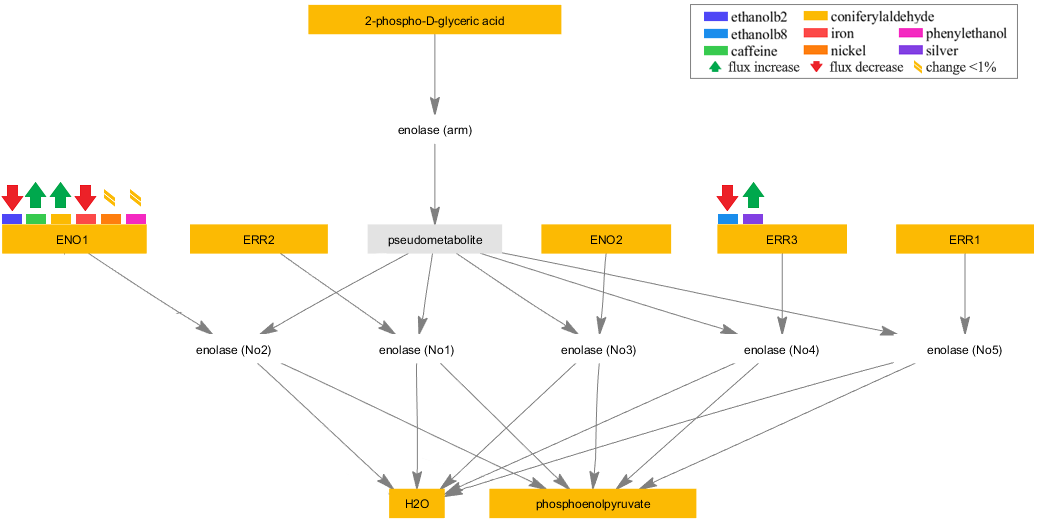
\includegraphics[width=1\columnwidth]{figures/discuss_enoerr.png}
\caption[Map of enolase catalyzed reaction as it used in simulations]{Map of enolase catalyzed reaction as it used in simulations. Corresponding genes used for evolved strains are shown in colors, and flux changes compared to reference strain model simulations are indicated as increased or decreased with arrows.}
\label{fig:discuss_ENOERR}
\end{figure}

\vspace{-0.5cm}

The phosphoglycerate mutase, another enzyme that caused distance between the simulations of evolved strains, is associated with the tetrameric GPM1 (YKL152C), and Q12040 (YOR283W) genes. It catalyzes the conversion of 3-phosphoglycerate to 2-phosphoglycerate in glycolysis pathway (step 8), and also the reverse reaction during gluconeogenesis. GPM1 and Q12040 have similarities in functioning as phosphoglycerate mutases, however Q12040 is a phosphatase with broader substrate specificity \cite{ho2009identification}. Studies on animals have shown that phosphoglycerate mutase activity is sensitive ionic concentration, such as high concentration of salts inhibit its mutase activity \cite{grisolia1967mercury}.

The fold change values of the gene GPM1 from differential analysis indicated an upregulation for ethanol-B8 and phenylethanol resistant, and a downregulation for silver resistant strain. No differential change is detected in the remaining resistant strains. For the enzyme Q12040, most of the strains showed downregulation, except an upregulation in silver resistant strain, and no change in ethanol-B2 and nickel resistant strains. In the FBA results, however, it is observed that all the models carry fluxes through the enzyme Q12040, while only the silver resistant strain uses the enzyme GPM1. These oppositions put forth the importance of the integrity of metabolic systems, and promotes to investigate systems as a whole instead of considering single values.
\begin{figure}[H]
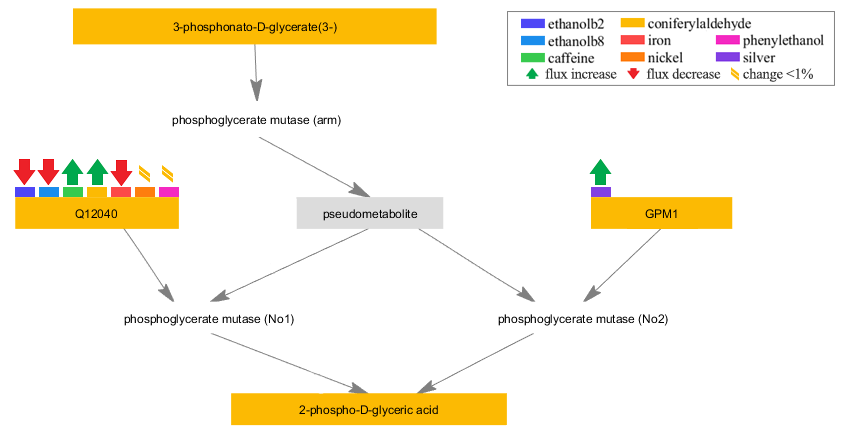
\includegraphics[width=1\columnwidth]{figures/discuss_PMG.png}
\caption[Map of phosphoglycerate mutase catalyzed reaction as it used in simulations]{Map of phosphoglycerate mutase catalyzed reaction as it used in simulations. Corresponding genes used for evolved strains are shown in colors, and flux changes compared to reference strain model simulations are indicated as increased or decreased with arrows.}
\label{fig:discuss_PMG}
\end{figure}
\vspace{-0.5cm}

\section{Strain Survivability}
\emph{In-silico} knock-out simulations showed that the single deletions of the enzymes L-homoserine-O-acetyltransferase (MET2), heme A:farnesyltransferase (COX10), gamma-aminobutyrate transaminase or 4-aminobutyrate aminotransferase (UGA1), succinate semialdehyde dehydrogenase (UGA2), protoporphyrinogen oxidase (HEM14), thiamine-phosphate diphosphorylase and hydroxyethylthiazole kinase (THI6), and 5'-methylthioribose-1-phosphate isomerase (MRI1) are essential for the growth of all evolved strains except caffeine resistant strain which is totally unaffected by the deletions of mentioned enzymes. From those, THI6 that is required for thiamine biosynthesis is already reported essential in the literature \cite{nosaka1994isolation}, however the caffeine resistant strain was able to grow at even higher rates without it.

Contrarily, the caffeine resistant strain decreased its growth rate by half when the enzymes 3-phosphoglycerate kinase (PGK1), $\beta $-subunit of heterooctameric phosphofructokinase (PFK2), triose phosphate isomerase (TPI1), and phosphoglucose isomerase (PGI1) are blocked (knocked-out), whereas the other strains could survive without getting affected much.

Another contrast is observed when the uroporphyrinogen-III synthase (HEM4) is deleted. Uroporphyrinogen III synthase catalyzes the conversion of preuroporphyrinogen to uroporphyrinogen-III in the fourth step in heme biosynthesis\cite{amillet1995isolation}. Although it is not reported as essential in literature, its deficiency can result in the diseases in the human homolog \cite{tan2008identification}. In survivability analysis simulations, ethanol B8, caffeine, and phenylethanol resistant strains did not affected from its deletion, however other strains could not grow at all.

Single deletions showed that all the evolved strains including the reference strain could not produce biomass at high rates when S-adenosylmethionine synthetase (SAM1) and protein O-mannosyltransferase (PMT5). SAM1 catalyzes the transfer of adenosyl group from ATP to L-methionine, forming S-adenosyl-L-methionine \cite{chiang1977activation}, and PMT5 catalyzes the release of mannose residues from dolichyl D-mannosyl phosphate in the endoplasmic reticulum \cite{girrbach2003members}. Although these enzymes are not found as essential, biomass production occurred despite the low rates, they are found as highly required by all strains therefore forming a common behavior across evolved strains.

\section{Simulations vs. Experimental Results}
Turanlı-Yıldız et al., obtained two evolved clones that could tolerate up to 12\% (v/v) ethanol, namely B2 and B8 strains, under increasing ethanol levels \cite{TuranlYldz2017}. Apart from the important findings on triggered diploidization during adaptation, their transcriptome analyses revealed that the most enriched genes were related to carbohydrates storage metabolism, however, only B2 strain alone exhibited a higher glycogen accumulation. They have also found that the abundances of mitochondrial proteins were decreased in B8 strain, suggesting a reduced respiratory activity. On top of that, findings on higher abundances of ribosomal proteins, amino acid metabolism, and glycolysis supported the idea of a higher fermentation levels.

\emph{in-silico} simulations show that, under the same environmental conditions provided, B2 strain is able to grow at slightly higher rates compared to B8 strain, 0.347 h\textsuperscript{-1} and 0.337 h\textsuperscript{-1} respectively, while B8 strain is able to produce ethanol at a higher rate 10.667 mmol/gDWh\textsuperscript{-1} compared to 9.934 mmol/gDWh\textsuperscript{-1} for B2 strain. The main difference observed in simulations between B2 and B8 strains is the regulation of citrate in the TCA cycle, specifically the transport reaction,
\begin{align}
\label{eq:citratetransport}
\ citrate_c + isocitrate_m \xleftrightarrow[\text{Rev: B8 (0.319 mmol/gDWh\textsuperscript{-1})}]{\text{Fwd: B2 (0.218 mmol/gDWh\textsuperscript{-1})}} citrate_m + isocitrate_c
\end{align}
\noindent where the indicators \emph{c} is for the cytoplasmic, and \emph{m} is for the mitochondrial metabolites. Transportation of citrate from mitochondria to cytoplasm in B8 strain agrees with the experimental findings on the idea of reduced respiratory activity, and this idea is supported with the ferrocytochrome-c:oxygen oxidoreductase (oxidative phosphorilation) fluxes where B2 strain has higher flux rate 18.867 mmol/gDWh\textsuperscript{-1}, compared to 17.439 mmol/gDWh\textsuperscript{-1} on B8 strain.

Although there is not a clear indicator on the glycogen synthase on simulations, the reason behind a slightly higher growth rate for B2 strain could arise from the carbohydrate pseudoreaction,
\begin{align}
\begin{split}
\  0.74851 \text{ (1-3)-beta-D-glucan} + 0.25009 \text{ (1-6)-beta-D-glucan } + \\
\ 0.36141 \text{ glycogen} + 0.71094 \text{ mannan} + 0.13828 \text{ trehalose} \xrightarrow{}  \text{carbohydrate}
\end{split}
\end{align}
required for biomass. However, it must be noted that only 0.003 mmol/gDWh\textsuperscript{-1} difference is observed between B2 and B8 clones for the glycogen (starch) synthase reaction where UDP-D-glucose is converted into glycogen.

Sürmeli et al., obtained yeast populations that can survive at high caffeine levels \cite{Srmeli2019}. Contrary to expectations from literature, their evolved strain, Caf905-2, did not show any inhibitory effects on the growth during stress selection. Transcriptome analysis on the obtained evolved strain, showed that Cytochrome c isoform 2 (CYC7) was the most upregulated gene. It is known that CYC7 is an electron carrier of the mitochondrial intermembrane space, and it is expressed under hypoxic conditions. In our simulations, we were able to catch the over-expression of CYC7 on flux variability analysis (Table \ref{table:fva_results}). As mentioned before, caffeine resistant strain reaches to highest growth rate among evolved strains, and it was able to maintain energy without oxidative phosphorylation. As it can be seen from the phenotype phase planes in Figure \ref{fig:robustness_glu_oxy}, caffeine resistant strain is highly sensitive oxygen availability and cannot grow if the oxygen uptake rate is higher than 25 mmol/gDWh\textsuperscript{-1}. Flux balance analysis shows that caffeine resistant strain reaches its maximum available growth rate of 0.468 h\textsuperscript{-1} when the oxygen uptake rate is 0.235 mmol/gDWh\textsuperscript{-1}. In other words, the model chooses not to take oxygen from outside if the carbon supply is unlimited in the media, it simulates hypoxic conditions for best outcome. However, if the glucose uptake is forced to 10 mmol/gDWh\textsuperscript{-1}, model takes more oxygen at the rate 4.757 mmol/gDWh\textsuperscript{-1}.

In their work, it has also been reported the induction of genes involved in glycogen and trehalose metabolism under caffeine stress. However, since the genome-scale modelling does not simulate stress conditions (i.e., no caffeine molecule is provided into the defined medium), this finding is not observed in the simulations, suggesting that this change could be regulated on the metabolic level, not on the transcriptomics level. Additionally, upregulation of SNQ2 was also not captured in the simulations, due to lack of its gene association in the Yeast8 model.

Transcriptomic changes in a coniferyl aldehyde resistant yeast population, BH13, is reported by Hacısalihoğlu et al., and differential regulations after adaptive evolution on the NAD(P)-dependent aldehyde dehydrogenases are revealed. They reported that all members of aldehyde dehydrogenases (ALD) except for ALD5 were upregulated, and ALD upregulation were previously observed in the literature \cite{adeboye2015catabolism}. Additionally, oxidoreductase enzymes such as BDH2, YPL113C, YJR096W; and putative aryl-alcohol dehydrogenases such as YPL088W and AAD15 were reported as upregulated in coniferyl aldehyde resistant strain. Here, in flux variability analysis, ALD4 upregulation is observed in coniferyl aldehyde resistant strain, accompanied with the caffeine and phenylethanol resistant strains.

In the coniferyl aldehyde resistant strain, Hacısalihoğlu et al. reported that the glucose uptake and metabolism were enhanced even without the coniferyl aldehyde stress in the media \cite{Hacsaliholu2019}. This observation is explained by the upregulation of the genes encoding hexose transporters, and the enzymes involved in glycolysis, namely HXK1, GLK1, TDH1, GPM2, ERR1, and PYK2. Increased glucose uptake compared to wild-type model, and high flux range on flux variability analysis for HXK1, GLK1, and PYK2 in coniferyl aldehyde resistant strain confirms \emph{in-silico} simulations to the experimental findings. Similar to the results of ADL family, GLK1 enzyme has a higher flux range in caffeine and phenylethanol resistant strains next to coniferyl aldehyde resistant strain. Interestingly, for the flux range of PYK2, iron resistant strain accompanies coniferyl aldehyde and caffeine resistant strains instead of phenylethanol resistant strain.


Iron resistant \emph{S. cerevisiae} mutant, M8FE, is obtained by Balaban et al with cross resistance feature to other metals \cite{balaban2020evolutionary}, and their findings suggested that the resistance to the metals might be related to the downregulation of PHO84 gene, encoding a high-affinity inorganic phosphate transporter and also a low-affinity manganese transporter. Unfortunately, phosphate uptake rates show no significant difference on \emph{in-silico} simulations. In the experiments, it is assumed that high amounts of iron would lead to oxidative stress that damage the cells, however, ROS amounts of the evolved M8FE strain were lower compared to reference strain. This phenomenon explained with the microarray results, where the upregulation on the oxidative stress response genes were observed. This upregulation is assumed to achieved in order to reduce oxidative levels in the cell. In the simulations, iron resistant strain was able to grow at the same rate with the reference strain model when the maximum glucose uptake is allowed (Table \ref{table:growth_glucose_table}). However, when we consider ATP production, despite having high glucose uptake and growth rates as reference strain model, iron resistant strain has much lower fluxes through ATP producing reactions compared to other models (Figure \ref{fig:fba_gro_glu_atp}). Although there is no \emph{in-silico} confirmation, Balaban et al. suggests that the iron resistant strain prefers to save its energy as trehalose in the cell.

Their study also reported upregulations on the glycogen phosphorylase gene, GPH1; and phosphoglucomutase, PGM2. Here, flux variability analyses showed a high range for all evolved strains for the enzyme PGM2, catalyst of the conversion from glucose-1-phosphate to glucose-6-phosphate, except in the silver resistant strain. That being said, the upregulation in the PGM2 might possibly be related to DNA replication stress, and not a specific upregulation for the metal stress.

Küçükgöze et al. obtained nickel resistant strain of \emph{S. cerevisiae}, called M9, with applications of ethyl methane sulfonate mutagenesis, and pulse stress of NiCl$_2$ in the media \cite{kuccukgoze2013evolutionary}. Their results show upregulations on metal homeostasis, especially iron metabolism, and stress response genes upon nickel exposure. Since we were able to integrate only 28 differentially expressed genes to build nickel resistant strain, its simulation results were similar to reference strain model simulations. Despite this, the nickel resistant strain showed 2.4-fold increase on the flux for MET2 gene which codes for homoserine O-acetyltransferase, followed by 1.5-fold increase on PFK2 (ATP-dependent 6-phosphofructokinase subunit beta), PDX1 (mitochondrial pyruvate dehydrogenase complex protein X component), and ARG7 (mitochondrial arginine biosynthesis bifunctional protein ArgJ).

Lastly, the silver resistant strain 2E were obtained by Terzioğlu et al. by using evolutionary engineering \cite{terziouglu2020genomic}. They showed the strain 2E has cross-resistance to copper, as both transition metals are similar, and copper-binding protein encoding genes are upregulated (such as CUP1-1, CUP1-2, and CTR3). Interestingly, they showed that their silver resistant strain has different mitochondrial activities compared to previous studies by Horstmann et al.\cite{horstmann2019transcriptome}, and Marquez et al. \cite{galvan2018zinc} in terms of mitochondrial activities. It has been shown by previous studies that silver stress causes decreased cellular respiration, and increased oxidative stress. However, Terzioğlu et al. reported an upregulation on set of genes encoding proteins for electron transfer system (such as CYC7, COX7, NDI1, and SDH1) indicating a higher activity on aerobic respiration. Additionally, GPX1, GRX1, and GRX2 genes were also reported as upregulated.

Although differential expressions of the study of Terzioğlu et al. were used to obtain silver resistant strain, our analysis results were in agreement with the previous findings. Simulations show zero flux through oxidative phosphorylation in mitochondria, despite having the second highest glucose uptake and ATP production flux rates. Genes that are upregulated in the differential analysis, namely GPX1, GRX1 and GRX2, were not used by the silver resistant strain, i.e., carried zero fluxes.
